%%%%%%%%%%%%%%%%%%%%%%%%%%%%%%%%%%%%%%%%%%%%%%%%%%%%
\section{Experimental Environment}\label{sec:eva-env}
%%%%%%%%%%%%%%%%%%%%%%%%%%%%%%%%%%%%%%%%%%%%%%%%%%%%

All the experiments in this paper are executed on the NERSC Edison
Cray XC30 supercomputer. Each node of Edison composes of 64~GB of DDR3
memory with two sockets, each socket is populated with a 12-core
% Intel\textsuperscript{\circledR} Xeon\textsuperscript{\circledR} E5-2695
v2 processors (Ivy Bridge), with running 19.2 GFLOPS\slash core performance.
The Cray Aries interconnect with Dragonfly topology is employed as the
interconnect of Edison, leveraging up to 8 GB\slash s MPI bandwidth
and 1.3 $\mu$s internode MPI latency.

The Intel compiler Composer XE 2015.1.133 and the Cray MPI 7.2.1 are used
for all the experiments. For NWChem evaluation, we use NWChem version 6.3
with MKL 11.2.1 as the external math library. We note that the Cray MPI
contains a {\em regular mode} and a {\em DMAPP mode}.
The {\em regular mode} executes all RMA operations in software with
asynchronous progress possible through background threads (by setting
the \fn{MPICH\_ASYNC\_PROGRESS} environment variable); the {\em DMAPP mode}
executes contiguous PUT and GET operations in hardware and provides
interrupt-based asynchronous progress for other operations (i.e., accumulate,
noncontiguous operations).
Since in the previous work, we have observed significant overhead of
frequent interrupts in the {\em DMAPP mode} that can be difficult to
benefit real applications, we only compare Casper with the {\em regular mode}
in this paper.


%%%%%%%%%%%%%%%%%%%%%%%%%%%%%%%%%%%%%%%%%%%%%%%%%%%%%%%%%%%%%%%%%%%%%%
\section{NWChem with Static Casper}\label{sec:eva-nwchem}
%%%%%%%%%%%%%%%%%%%%%%%%%%%%%%%%%%%%%%%%%%%%%%%%%%%%%%%%%%%%%%%%%%%%%%
In our previous work, we have demonstrated significant performance
improvement of large chemistry application NWChem with the static Casper
for the C$_{20}$ problem and a very large water molecule (H$_2$O)$_{20}$
in the CCSD(T) simulation~\cite{casper}\cite{casper-scaling}. However,
we did not understand the exact performance change in each internal
phases. To exploit the maximum performance improvement, we need a deep
study to characterize the performance of NWChem internal phases with
varying asynchronous progress approaches.
In following sections, we first give an overview of the NWChem application,
then we deeply analyze the performance characteristics of the internal
phases of the CCSD(T) simulation with two different problem types, a
Water molecule ((H$_2$O)$_n $) series, and an Acenes series.

%%%%%%%%%%%%%%%%%%%%%%%%%%%%%%%%%%%%%%%%%%%%%%%%%%%%
\subsection{NWChem Overview}\label{sec:eva-nwchem-overview}
%%%%%%%%%%%%%%%%%%%%%%%%%%%%%%%%%%%%%%%%%%%%%%%%%%%%
NWChem~\cite{NWChem63} is a computational chemistry application suite
offering many simulation capabilities, with providing extensive
functionality~\cite{Hirata:2003:JPCA:TCE} and excellent
performance~\cite{Apra:2009:SC:NWChem}. NWChem is developed on top
of the Global Arrays~\cite{GA_SC94} toolkit, which provides an abstraction
of global shared array that hides the complexity of domain distribution
across physical nodes. It is implemented on a number of platforms
natively and as a portable implementation over MPI
RMA~\cite{dinan12:armci_mpi}.

The coupled cluster (CC) theory is one of the most popular approaches
in quantum chemistry for solving electron correlation in atoms and
molecules with arbitrary accuracy requirements. NWChem provides highly
efficient parallel implementations for a variety of complicated CC methods
through the Tensor Contraction Engine (TCE). The ``gold standard''
{\em coupled cluster with singles and doubles and perturbative triples}
method, known as CCSD(T), is one of the most accurate CC methods
applicable to large molecules to date. It is particularly useful for
calculating accurate noncovalent interaction energies.

\begin{algorithm}
\caption{Generic get-compute-update mode in NWChem.}
\label{code:ccsd-get-comp-up}
Global Arrays: A, B, C\;
Local Buffers : a, b, c\;
\For {each sub block in A, B}{
    GET $a$ from $A$\;
    GET $b$ from $B$\;
    COMPUTE $c = a \times b + c$\;
    UPDATE $c$ to $C$\;
    NXTASK;
}
\end{algorithm}

The {\em get-compute-update} mode is the generic code structure used
in all the internal phases of NWChem, which performs large
three-dimensional matrix--matrix multiplications. As demonstrated in
Algorithm~\ref{code:ccsd-get-comp-up}, in the {\em get-compute-update}
mode, each processes first gets sub-domain $a$ and $b$ from global
arrays that are located in the memory spaces of remote processes, then
performs a local DGEMM and next it updates the result $c$ back to the
global memory, accumulating the values. The nxtask module is called
after every sub-domain computation to decide the computing process
for the next computation.

The CCSD(T) method performs a complex set of multidimensional
array computations organized in three internal phases: four-index
transformation (4-index), CCSD iteration, and the noniterative (T)
portion~\cite{CPE:CPE1881}.

\parasubhead{Four-index transformation}:
The 4-index phase requires a number of DGEMM computation with a
non-collective global transpose in the middle, containing intensive
PUT/GET/ACCUMUALTE communication following the {\em get-compute-update}
mode.

\parasubhead{CCSD iteration}:
This phase evaluates the residual for the complex set of
nonlinear CCSD equations. Each of the iterative steps composes of window
allocation, a number of global synchronization calls and the typical
{\em get-compute-update} loop that involves large amount of
GET operations and a number of ACCUMULATE operations with DGEMM
computation.

\parasubhead{(T) portion}:
In the noniterative (T) portion phase, every process only perform
one large matrix--matrix multiplication also following the typical
{\em get-compute-updates} approach, containing large COMPUTE operations
with numerous GET operations and a reduce operation (update) at
the end of local multiplication.

All the above phases contain the nxtask module, in which processes
issue atomic FETCH\_AND\_OP operation on a global shared counter to
schedule the computation for the next sub-domain.


%%%%%%%%%%%%%%%%%%%%%%%%%%%%%%%%%%%%%%%%%%%%%%%%%%%%
\subsection{Experiments Overview}
%%%%%%%%%%%%%%%%%%%%%%%%%%%%%%%%%%%%%%%%%%%%%%%%%%%%

We evaluated the improvement of NWChem by comparing the static Casper
with both the original MPI and two thread-based approaches. The first
Thread~(O) approach employs oversubscribed cores where every thread and
its associated MPI process execute on the same core; and the second
Thread~(D) approach deploys dedicated cores where threads and MPI
processes are executed on separate cores. We use the same total number
of cores in all approaches, some of which are dedicated to asynchronous
ghost processes\slash threads as listed in Table~\ref{tab:eva-csp-nwcore}.

\begin{table}%\scriptsize
\begin{center}
\caption{Core deployment in NWChem evaluation on Cray XC30.}\label{tab:eva-csp-nwcore}
\begin{tabular}{|c|cc|}
% \hline
\hline
& Computing Cores & ASYNC Cores \\
\hline
Original MPI & 24 & 0 \\
Casper (1) & 23 & 1 \\
Casper (2) & 22 & 2 \\
Casper (4) & 20 & 4 \\
Casper (8) & 16 & 8 \\
Thread (O) & 24 & 24 \\
Thread (D) & 12 & 12 \\
\hline
% \hline
\end{tabular}
\end{center}
% \vspace{-4.0ex}
\end{table}

Different from the experiments in our previous works, we use the NTS task
scheduling module in all of our experiments in this paper by adding
``set tce:nts T'' in the input files. The NTS module significantly reduces
the overhead of nxtask scheduling especially in the CCSD iteration.


%%%%%%%%%%%%%%%%%%%%%%%%%%%%%%%%%%%%%%%%%%%%%%%%%%%%
\subsection{CCSD(T) with Water Molecules}\label{sec:eva-nwchem-basic-ccsdt}
%%%%%%%%%%%%%%%%%%%%%%%%%%%%%%%%%%%%%%%%%%%%%%%%%%%%

In this section, we focus on the CCSD(T) method with water molecule
problems ((H$_2$O)$_n$)---denoted W$_n$ for short---with double-zeta
basis sets (cc-pVDZ from the NWChem basis set library).

To have a global view of the performance effect caused by different
asynchronous progress approaches, we first evaluated Casper with
comparison of both the original MPI and thread-based approaches in
weak scaling. Figure~\ref{fig:eva-edison-nw-ccsdt-wN} indicates the task
time of CCSD(T) method for varying W$_n$-pVDZ problems
($n=5, 10, 14, 16, 18, 21$). Casper consistently improves the performance
from problem W$_{10}$ to W$_{21}$ by close to 30\%. However, the
thread-based approaches do not show performance improvement and perform
even worse than the original MPI because of oversubscribed cores or
appropriation of half of the computing cores. We notice that Casper
shows 15\% performance degradation in W$_{5}$, which is executed on only
single node. This is because MPI internally allocates shared window for
the processes on the same node, thus all the RMA operations are handled
in hardware through the shared memory. Casper does not degrade the
performance of communication, however, it takes 4 cores from the user
computation.

\begin{figure}
\centering
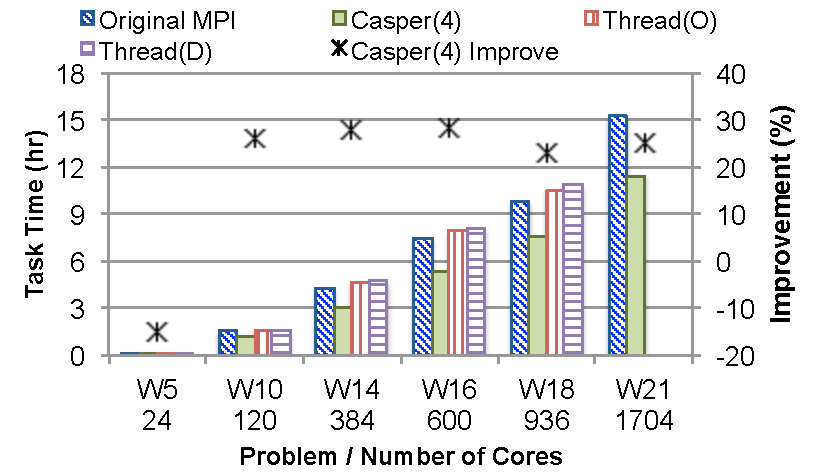
\includegraphics[width=0.8\columnwidth]{figures/adpt-casper/eva_edison_nw_wn_ccsd_t_task_weak.pdf}
\caption{CCSD(T) for varying W$_n$ with pVDZ on Cray XC30.\mynote{add W21-threads.}}
\label{fig:eva-edison-nw-ccsdt-wN}
\end{figure}

\begin{figure}
\centering
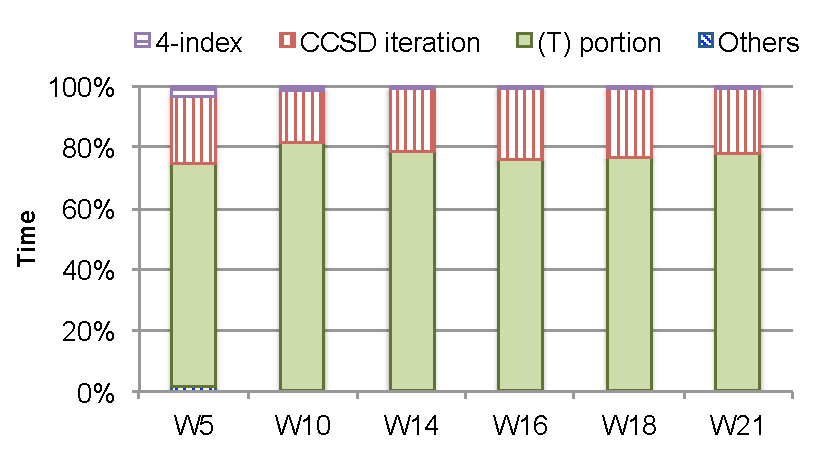
\includegraphics[width=0.8\columnwidth]{figures/adpt-casper/eva_edison_nw_wn_ccsd_t_steps_weak.pdf}
\caption{Task internal phases in varying W$_n$ with pVDZ on Cray XC30.}
\label{fig:eva-edison-nw-ccsdt-wN-pf}
\end{figure}

To investigate the impact of asynchronous progress on each internal
phase, we next measured the time consumed by each phase for the CCSD(T)
task. As we have described in Section~\ref{sec:eva-nwchem-overview}, the
CCSD(T) method consists of three primary internal phases, 4-index, CCSD
iteration and (T) portion. As shown in Figure~\ref{fig:eva-edison-nw-ccsdt-wN-pf},
the (T) portion consistently dominates the cost of entire task by close
to 80\% for all the water problems, and the CCSD iteration takes the
other 20\%; the 4-index and other internal phases represent less than
2\% of the execution time. Therefore, we only focus on the analysis of
the CCSD iteration and the (T) portion phases.

%%%%%%%%%%%%%%%%%%%%%%%%%%%%%%%%%%%%
\subsubsection{CCSD Iteration Phase}
%%%%%%%%%%%%%%%%%%%%%%%%%%%%%%%%%%%%

Figure~\ref{fig:eva-edison-nw-ccsd-w21-1704-pf} shows the profiling of
the communication-dominative CCSD iteration phase in the W$_{21}$-pVDZ
problem with 1704 cores. The numerous GET operations dominate the execution
time by close to 80~\%, while the DGEMM computation (shown as COMP) only
takes less than 10~\% of the cost and the FETCH\_AND\_OP (abbreviated to FOP)
almost takes the rest 10~\%.

Such intensive communication can rarely benefit from the asynchronous
progress, however, can even result in performance degradation.
When only a single ghost process is used within Casper, the overhead of
GET operation becomes twice more expensive than the original MPI,
because a large amount of GET operations, which were distributed to 24
user processes on each node, are redirected to a single ghost process,
thus resulting in the bottleneck of communication load imbalance. With
utilizing more ghost processes, this imbalance issue is resolved, however,
the overhead the DGEMM computation slightly increases due to loss of
computing cores.

\begin{figure*}
\centering
\subfigure[CCSD iteration]{
  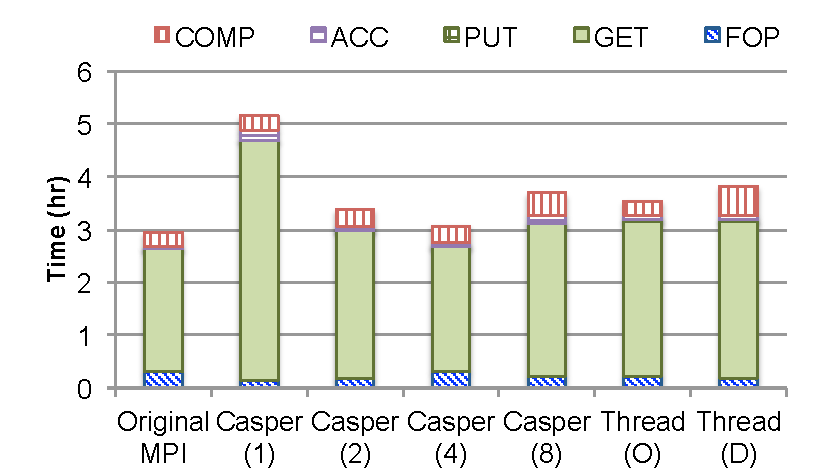
\includegraphics[width=0.64\columnwidth]{figures/adpt-casper/eva_edison_nw_w21_ccsd_t_n1704_ccsd_steps.pdf}
  \label{fig:eva-edison-nw-ccsd-w21-1704-pf}
}
\subfigure[(T) portion \mynote{update with v721-mkl}]{
  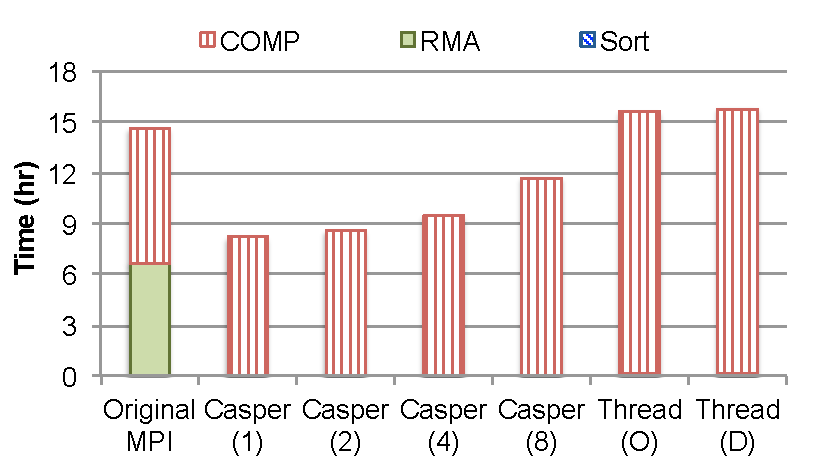
\includegraphics[width=0.64\columnwidth]{figures/adpt-casper/eva_edision_nw_w21_ccsd_t_n1704_t_steps.pdf}
  \label{fig:eva-edison-nw-ccsdt-w21-t-1704-pf}
}
\subfigure[Trade off between CCSD iteration and (T)\mynote{update with v721-mkl}]{
  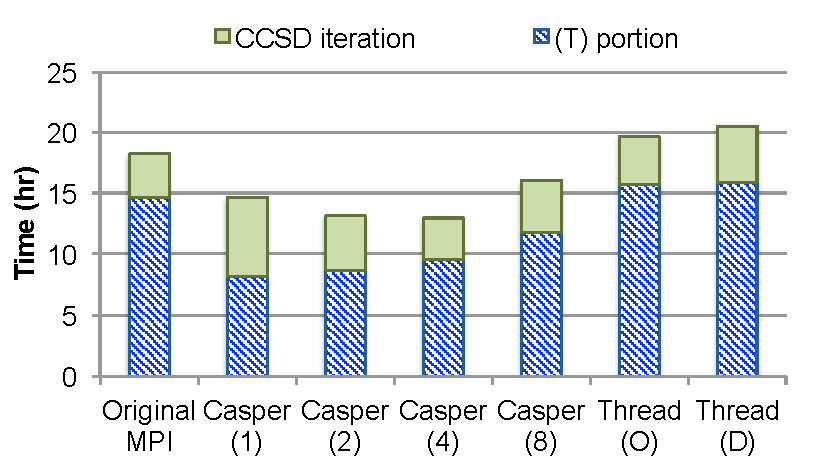
\includegraphics[width=0.64\columnwidth]{figures/adpt-casper/eva_edision_nw_w21_ccsd_t_n1704_steps.pdf}
  \label{fig:eva-edison-nw-ccsdt-w21-pf}
}
% \vspace{-1.0ex}
\caption{Profiling CCSD iteration and (T) portion for W21 problem with 1704 cores on Cray XC30.}
\label{fig:eva-nwchem-w-prof}
% \vspace{-4.0ex}
\end{figure*}


%%%%%%%%%%%%%%%%%%%%%%%%%%%%%%%%%%%%
\subsubsection{(T) Portion Phase}
%%%%%%%%%%%%%%%%%%%%%%%%%%%%%%%%%%%%

We next profile the most time-consuming phase: (T), which also follows the
typical {\em get-compute-update} approach containing extremely heavy
matrix-matrix multiplication computations (COMP) with numerous GET operations.
Figure~\ref{fig:eva-edison-nw-ccsdt-w21-t-1704-pf} shows the time consumed
in the internal steps of (T) in W$_{21}$-pVDZ problem with 1704 cores.
In the result of original MPI, the heavy computations takes 6.46~hours
and the GET communication dominates the other half of cost, taking
5.35~hours. The significant overhead of GET clearly indicates the delay
caused by heavy computation on the target processes when no asynchronous
progress is provided. Both Casper and the thread-based approaches asynchronously
handles the completion of GET operations thus the overhead of GET dramatically
reduced. However, within more number of ghost processes in Casper, the
computation part shows a performance degradation because of reduced
computation resources. Because of similar reason, the thread-based approach
with dedicated cores (Thread (D)) performs even worse than the original MPI
since half of the computing cores are dedicated to communication.


%%%%%%%%%%%%%%%%%%%%%%%%%%%%%%%%%%%%%%%%%%%%%%%
\subsubsection{Asynchronous Progress Trade-Off}
%%%%%%%%%%%%%%%%%%%%%%%%%%%%%%%%%%%%%%%%%%%%%%%

According to above profiling results, it is clear that the needs of
asynchronous progress is varying for different phases in a CCSD(T) task.
Figure~\ref{fig:eva-edison-nw-ccsdt-w21-pf} compares the time of CCSD
iteration and (T) with the thread-based approaches and the static Casper
with different number of ghost processes. Although the (T) portion gets
a great improvement by using only one ghost process, the performance of
the CCSD iteration shows a degradation because of load imbalance issue.
we demonstrated in Figure~\ref{fig:eva-edison-nw-ccsd-w21-1704-pf}. Hence,
to achieve the optimal performance for the entire task, we need trade off
among these internal phases that require different number of asynchronous
cores. For example, the optimal number of ghost processes for the W$_{21}$
problem is four on our platform.
% \mynote{briefly discuss CCSD method somewhere.} % not follow the story.

%%%%%%%%%%%%%%%%%%%%%%%%%%%%%%%%%%%%%%%%%%%%%%%%%%%%
\subsection{CCSD(T) with Acenes Molecules}
%%%%%%%%%%%%%%%%%%%%%%%%%%%%%%%%%%%%%%%%%%%%%%%%%%%%

As shown in above section, the CCSD(T) task requires different number of
ghost processes to obtain the optimal performance in CCSD iteration and (T)
potion phases separately. Thus a static configuration of asynchronous
progress can lead to insufficient performance improvement,  or even
performance degradation such as the performance loss in the CCSD iteration
phase while specifying only one ghost process.
For water problems, such insufficiency does not significantly
impair the performance of the entire execution of task, since the (T)
portion, whose performance could be improved by close to 50\%, dominates
the cost of entire task. However, this might not be true for other molecule
problems.

In this section, we look into the performance of Casper within the
acenes series including Naphthalene (C$_{10}$H$_{8}$),
Anthracene (C$_{14}$H$_{10}$), Tetracene (C$_{18}$H$_{12}$),
Pentacene (C$_{22}$H$_{14}$) and Hexacene (C$_{26}$H$_{16}$) molecules,
with \mynote{double-zeta basis sets} (aug-cc-pVDZ from the NWChem basis set
library), which show a different proportion for each internal phase in the
execution of CCSD(T) task. These problems are abbreviated to Nap, Ant, Tet,
Pent and Hexa respectively for convenient description.

Figure~\ref{fig:eva-edison-nw-ccsdt-acenes-weak} compares the execution
time of the internal phases in this problem series.
Comparing with the results observed in water system, the proportion of
(T) portion is significantly reduced, instead, the communication-intensive
4-index shows more overhead. For example, the (T) portion takes only 52\%
of the entire cost in the Tet problem, while the 4-index becomes more
expensive and takes close to 26\% of the cost, and the CCSD iteration
and other internal phases take the other 19\% and 3\% costs respectively.


\begin{figure*}[ht]
\centering
\subfigure[Internal phases in Acenes series with pVDZ]{
  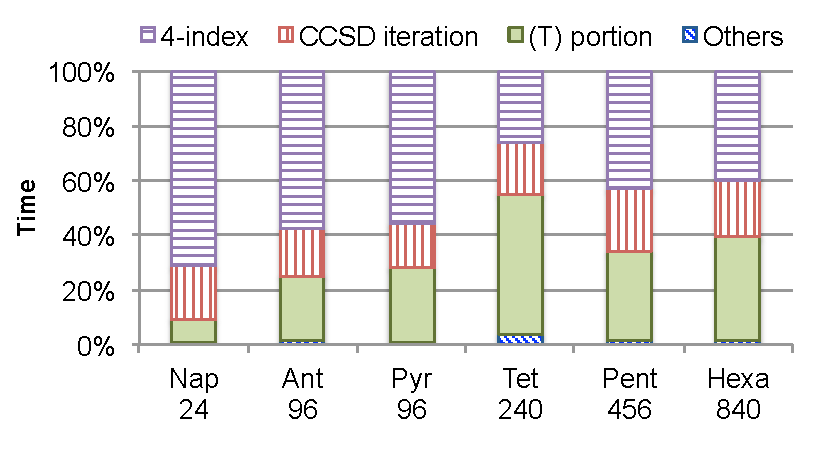
\includegraphics[width=0.64\columnwidth]{figures/adpt-casper/eva_edision_nw_acenes_ccsd_t_steps_weak.pdf}
  \label{fig:eva-edison-nw-ccsdt-acenes-weak}
}
\subfigure[Tet-pVDZ with 240 cores]{
  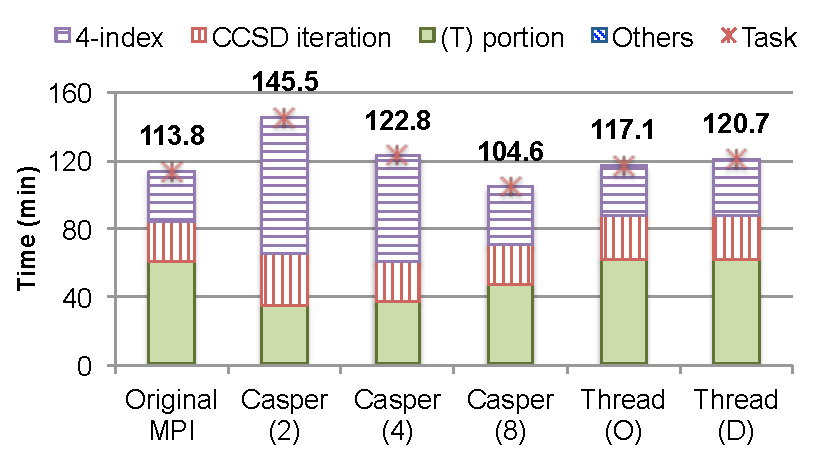
\includegraphics[width=0.64\columnwidth]{figures/adpt-casper/eva_edision_nw_tet_ccsd_t_n240.pdf}
  \label{fig:eva-edison-nw-ccsdt-tet-240}
}
\subfigure[Profiling of Tet-pVDZ on 240 cores]{
  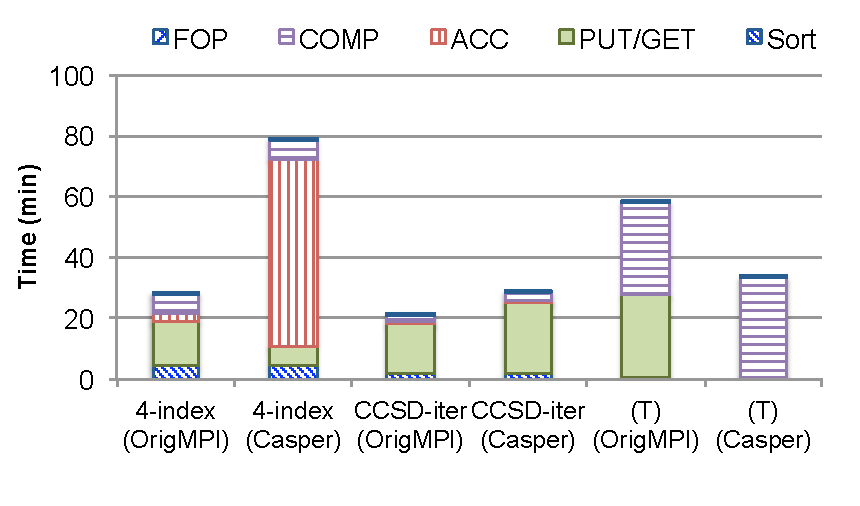
\includegraphics[width=0.64\columnwidth]{figures/adpt-casper/eva_edision_nw_tet_ccsd_t_n240_steps.pdf}
  \label{fig:eva-edison-nw-ccsdt-tet-240-pf}
}
\caption{CCSD(T) Task for acenes molecule on Cray XC30.}
\label{fig:eva-nwchem-acenes}
\end{figure*}

Since the proportion of communication-intensive phases is increased,
the performance degradation caused by static asynchronous progress in
those phases becomes more significant. We then focus on the Tet problem
running on 240 cores to demonstrate such inefficiency.
Figure~\ref{fig:eva-edison-nw-ccsdt-tet-240} compares the execution time
of thread-based approaches and static Casper with 2, 4 and 8 ghost processes
respectively. Unfortunately, neither Casper nor the thread-based approaches
can provide efficient solution for the Tet problem.
Although Casper can reduce the overhead of (T) portion by 40~\% when using
2 ghost processes, it also causes severe degradation of 4-index by close
to 160~\%, thus resulting in even worse performance of the entire task
execution. Withing increasing number of ghost processes, the degradation
of 4-index can be gradually resolved, however, (T) portion shows increasing
degradation because of loss of computing resources as studied in
Section~\ref{sec:eva-nwchem-basic-ccsdt}.

To ensure the reason causing different trend in these internal
phases, we also profiled the time-consuming 4-index, CCSD, and (T)
portion. Figure~\ref{fig:eva-edison-nw-ccsdt-tet-240-pf}
compares the performance of original MPI and that with Casper by using
2 ghost processes. As expected, Casper eliminates most overhead of
communication in the computation-intensive (T) portion; however,
the overhead of ACCUMULATE in 4-index step increases significantly,
thus resulting in performance degradation in 4-index. This is because
heavy ACCUMULATE communication which was received by 24 processes on
each node, has to be handled by only 2 ghost processes.
\mynote{why ACC is increased but PUT/GET is reduced ? Does it mean
COMP just performs together with PUT/GET ?}
